\documentclass[fleqn]{article}
%\textwidth=6in
%\textheight=9in
%\pagestyle{empty}
\usepackage{amsmath,amssymb,amsthm,ragged2e,siunitx,graphicx,multicol,wrapfig,mathtools,parskip}
\usepackage[margin=0.7in]{geometry}
\usepackage[T1]{fontenc}
\usepackage[utf8]{inputenc}
\usepackage[dvipsnames]{xcolor}
\usepackage[export]{adjustbox}
\newtheorem{thm}{{\sc Theorem}}[section]
\newtheorem{prop}[thm]{{\sc Proposition}}
\newtheorem{cor}[thm]{{\sc Corollary}}
\newtheorem{lem}[thm]{{\sc Lemma}}
\newtheorem{df}[thm]{{\sc Definition}}

\DeclarePairedDelimiter\ceil{\lceil}{\rceil}
\DeclarePairedDelimiter\floor{\lfloor}{\rfloor}

\DeclareMathOperator{\sech}{sech}
\DeclareMathOperator{\csch}{csch}

% automatically makes new paragraphs have no indent
\setlength{\parindent}{0pt}

\newcommand{\n}{\noindent}
\newcommand{\ds}{\displaystyle}
\newcommand{\rar}{\rightarrow}

% new command for underscore
\newcommand{\underscore}{\underline{\hspace{1cm}}}

% this is a command for the space between asterisk or plus and the problem statement
\newcommand{\gap}{\hspace{.25cm}}

\newcommand*\colvec[1]{\begin{bmatrix*}[r]#1\end{bmatrix*}} 

% Uncomment this to write vectors bolded 
\renewcommand{\vec}[1]{\boldsymbol{#1}}

% Uncomment this to write vectors bolded AND with arrow on top
\newcommand{\avec}[1]{\overrightarrow{\boldsymbol{#1}}}
% this notation has an arrow on top of vector which is redundant if it is bolded

% Uncomment this to write vectors unbolded with long arrow on top
% \renewcommand{\vec}[1]{\overrightarrow{#1}}

% this is a command for a coefficient matrix with right-aligned entries (good for aligning negative signs)
\newcommand{\mat}[1]{\begin{bmatrix*}[r]#1\end{bmatrix*}} 

% this is a command for a coefficient matrix with center-aligned entries (good for aligning negative signs)
\newcommand{\cmat}[1]{\begin{bmatrix*}[c]#1\end{bmatrix*}} 

% this is a command for a DETERMNINANT matrix with right-aligned entries (good for aligning negative signs) (ABSOLUTE VALUE BARS)
\newcommand{\vmat}[1]{\begin{vmatrix*}[r]#1\end{vmatrix*}} 

% this is a command for black squares (useful for pivots in matrices) when already in math mode (between $ signs)
\newcommand{\bsq}{\blacksquare}






%%  environment for AUGMENTED  matrices
\newenvironment{amatrix}[1]{%
  \left[\begin{array}{@{}*{#1}{r}|r@{}}
}{%
  \end{array}\right]
}


%%% new command for Augmented BAR alone (helpful for putting augmented bar somewhere in middle of matrix)
\newcommand\aug{\fboxsep=-\fboxrule\!\!\!\fbox{\strut}\!\!\!}

% define new color (i.e. pink)
\definecolor{mypink1}{rgb}{0.858, 0.188, 0.478}

% define new color (i.e. medium green)
\definecolor{MediumGreen}{rgb}{0.1, 0.8, 0.65}

% define new color (i.e. dark purple)
\definecolor{DarkPurple}{rgb}{0.6, 0, 0.6}

% this is a command for the size of headers
\newcommand{\header}[1]{\noindent{\Large \textcolor{mypink1}{\textbf{#1}}}}

% this is a command for the size of subheaders
\newcommand{\subheader}[1]{\noindent{\large \textcolor{red}{\textbf{#1}}}}

% this is a command for answers in RED on same line with a space between problem and answer
\newcommand{\sred}[1]{\hspace{1cm} \textcolor{red}{#1}}

% this is a command for answers in RED on same line with NO space between problem and answer
\newcommand{\red}[1]{\textcolor{red}{#1}}

% this is a command for answers in PURPLE on same line with NO space between problem and answer
\newcommand{\DarkPurple}[1]{\textcolor{DarkPurple}{#1}}

% this is a command for answers in GREEN on same line with NO space between problem and answer
\newcommand{\MediumGreen}[1]{\textcolor{MediumGreen}{#1}}

% this is a command for answers in BLUE on same line with a space between problem and answer
\newcommand{\sblue}[1]{\hspace{1cm} \textcolor{blue}{#1}}

% this is a command for answers in BLUE on same line with NO space between problem and answer
\newcommand{\blue}[1]{\textcolor{blue}{#1}}


% this is a command for defining EXAMPLES
\theoremstyle{definition}
\newtheorem{exmp}{Example}[section]




\begin{document}

\centerline{\Large \bf Math Seminar Template Notes}
\centerline{\large \bf Day 8 (Prove $\sqrt{2}$ is Irrational + Modular Arithmetic)}
\vspace{\baselineskip}

%\noindent \underline{\hspace{18cm}}

\header{Day 8 (Prove $\sqrt{2}$ is Irrational + Modular Arithmetic) } \\


\noindent\fbox{%
\parbox{\textwidth}{
\subheader{Overview} \\ 
%\vspace{0.25cm}
\textbf{\underline{Goals}} 
\begin{enumerate}
\item Prove $\sqrt{2}$ is irrational
\item Introduce modular arithmetic
\end{enumerate}
\vspace{.25cm}
}}

\vspace{0.2cm}

\subheader{$\sqrt{2}$ is Irrational}


%%%% something in a box
\noindent\fbox{%
\parbox{\textwidth}{\vspace{.25cm}
\textbf{Def:} A \textbf{rational} number is a real number that can be written in the form $\ds{\frac{a}{b}}$ where $a, b$ are integers and $b \neq 0$

\vspace{.25cm}
\hspace{1cm} \textbf{Examples:} \hfill $\ds{\frac{2}{5}}$ \hfill $\ds{-\frac{13}{7}}$, \hfill $\ds{0.25 = \frac{1}{4}}$, \hfill $\ds{0.333 \ldots = \frac{1}{3}}$ \hfill \hspace{.5cm}

\vspace{.5cm}
\textbf{Def:} An \textbf{irrational} number is a real number that is NOT rational. 

\vspace{.25cm}
\hspace{1cm} \textbf{Examples:} \hfill $\pi$ \hfill $e$ \hfill $\sqrt{3}$ \hfill $\ds{ \frac{\sqrt[3]{7}}{4} }$ \hfill \hspace{.5cm}

\vspace{.25cm}   
}}
%%% end box

\vspace{.25cm}
\textbf{Ex 1:} \textbf{Pf:} Assume for the sake of contradiction that \underline{\hspace{4.5cm}}. 

\vspace{.25cm}

Then, $\sqrt{2} = \hspace{1cm}$ for some $a, b \in \underline{\hspace{1cm}}, \ b \underline{\hspace{1.5cm}}$. Suppose \hspace{1cm} is written in lowest terms.

\vspace{.25cm}
{\it \textbf{Q:} What can you say about $a^2$?}

\vspace{2cm}
\hspace{7cm} This means $a^2$ is \underline{\hspace{2cm}} since $a^2 = $\underline{\hspace{1.5cm}} and \underline{\hspace{1.5cm}}. 

\vspace{.5cm}
Recall that $a^2$ is \underline{\hspace{2cm}} if and only if $a$ is \underline{\hspace{2cm}}. Thus, in our problem, \underline{\hspace{3.5cm}}, 

\vspace{.25cm}
so $a= \underline{\hspace{1.5cm}}$ for some \underline{\hspace{1.5cm}}. 

\vspace{.25cm}
{\it \textbf{Q:} What can we now do with this expression for $a$ along with our earlier knowledge that $a^2=2b^2$? }

\vspace{3cm}
% Substituting \underline{\hspace{2cm}} into \underline{\hspace{2cm}}, we get 

% \vspace{.5cm}
\hspace{6.5cm} This means $\underline{\hspace{1cm}}$ is \underline{\hspace{2cm}} since \underline{\hspace{2.5cm}} and \underline{\hspace{1.5cm}}

\vspace{.25cm} 
Since $a$ and $b$ are both \underline{\hspace{2cm}}, this means $\ds{\frac{a}{b}}$ is \underline{\hspace{7cm}} 

\vspace{.25cm}
This is a contradiction, and it follows that $\sqrt{2}$ is indeed irrational! 



%%%
\newpage

\subheader{Formalizing Divisibility}

%%%% something in a box
\noindent\fbox{%
\parbox{\textwidth}{\vspace{.25cm}
Note that $3$ \textbf{divides} $18$ which means $\displaystyle{\frac{18}{3}} = \underline{\hspace{1cm}}$ is an \underline{\hspace{3cm}}. Equivalently, $18 = 3(\hspace{.75cm})$

\vspace{.5cm}
\textbf{Def}: Let $a, b \in \mathbb{Z}$ with $a \neq 0$. We say \textbf{$a$ divides $b$} (or \textbf{$b$ is a multiple of $a$}) if $b = a(\underline{\hspace{1cm}})$ such that \underline{\hspace{2cm}}

\vspace{.5cm}
\textbf{Notation:} \hspace{1.5cm} means ``$a$ divides $b$"
\vspace{.25cm}   
}}
%%% end box

\vspace{.25cm}

\textbf{Ex 1:} Answer \textbf{yes} or \textbf{no} to the following questions. Explain using the above definition. 

\vspace{.25cm}
(a) $6 \ |  -18$ 

\vspace{.5cm} 
(b) $-18 \ | \ 6$ 

\vspace{.5cm}
(c) $4 \ | \ 0$ 

\vspace{.5cm}
(d) $0 \ | \ 4$ \hspace{8cm} This is why $\displaystyle{\frac{4}{0} }$ is \underline{\hspace{3cm}}

\vspace{.75cm}
(e) $0 \ | \ 0$ \hspace{8cm} This is why $\displaystyle{\frac{0}{0} }$ is \underline{\hspace{3cm}}


\vspace{.75cm}
%%%% something in a box
\noindent\fbox{%
\parbox{\textwidth}{\vspace{.25cm}
\textbf{Thm}: Let $a, b, c \in \mathbb{Z}$ with $a, b \neq 0$. Then,

    \vspace{.25cm}
	\begin{enumerate}
	\item If $a \ | \ b$ and $a \ | \ c$, then $a \ | \ (b \pm c)$ 

    \vspace{.1cm}
	\item If $a \ | \ b$, then $a \ | \ bc$

    \vspace{.1cm}
	\item If $a \ | \ b$ and $b \ | \ c$, then $a \ | \ c$ \hspace{.25cm}
	\end{enumerate}
\vspace{.25cm}   
}}
%%% end box

\vspace{.25cm}

\textbf{Ex 2:} Prove part of (1) of the theorem above, namely prove that if $a \ | \ b$, and $a \ | \ c$, then $a \ | \ (b - c)$

\vspace{.25cm} 

%%% Scratch work for proof
\hspace{7cm} \MediumGreen{\underline{Scratch Work}}
\begin{multicols}{2} 
\hspace{4cm} \MediumGreen{\underline{Given/Know}} \columnbreak

\MediumGreen{\underline{Want to show}} 
\end{multicols}

\vspace{2.5cm} 




%%%
\newpage

\textbf{Pf:}


\vspace{10cm}

\subheader{Exploring Modular Arithmetic}

\begin{multicols}{2} 
\textbf{Ex 3:} Suppose that it is 4:00 currently. What time is it in 

\vspace{.25cm}
(a) 10 hours?

\vspace{1.5cm}
(b) 26 hours? 

\vspace{1.5cm}
(c) 100 hours? 

\vspace{1.5cm} 
\columnbreak 
%image aligned
%%
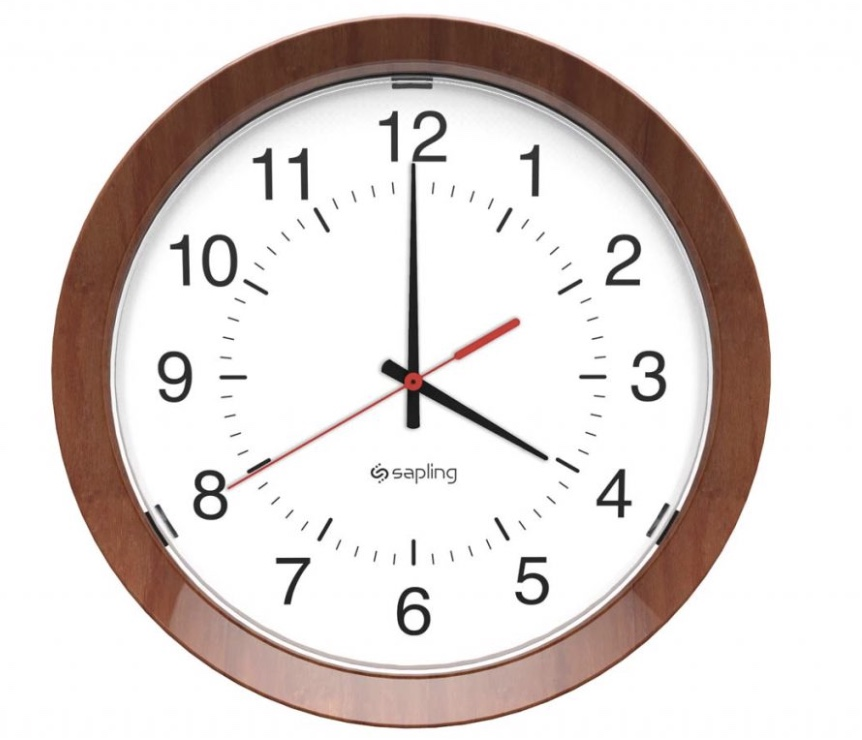
\includegraphics[scale=0.3, right]{Clock}
\vspace{-10pt}
\end{multicols}


%%%
\newpage


\textbf{Ex 4:} Find the remainder in the following division problems. 

\vspace{.25cm}
(a) $51$ is divided by $8$ 

\vspace{2cm} 
(b) $-51$ is divided by $-8$


\vspace{2cm}


%%%% something in a box
\noindent\fbox{%
\parbox{\textwidth}{\vspace{.25cm}
\textbf{Thm (Division Algorithm):} Let $a \in \mathbb{Z}$ and $d \in \mathbb{Z}^+$. There exist unique integers $q, r$ such that $$a=dq+r \text{ with } 0 \leq r \leq d-1$$

% \vspace{.25cm}
$q=$ quotient \hspace{1cm} $r=$ remainder \hspace{1cm} $d=$ divisor
\vspace{.25cm}   
}}
%%% end box

\vspace{.25cm}

%%%% something in a box
\noindent\fbox{%
\parbox{\textwidth}{\vspace{.25cm}
\textbf{Def \textbf{(Mod)}:} \DarkPurple{$a \mod m$} is the unique remainder when dividing $a$ by $m$. 
\vspace{.25cm}   
}}
%%% end box

\vspace{.25cm}

e.g. $51 \mod 8 = \underline{\hspace{1cm}}$ \hspace{1.5cm} $-51 \mod 8 = \underline{\hspace{1cm}}$

\vspace{.5cm}

``mod" is like \underline{\hspace{1cm}} in some programming languages

\vspace{.25cm}

\textbf{Note:} Clocks work in $\mod 12$ (or sometimes $\mod 24$). % For example, what will a 12-hr clock display 7 hours after 9:00? 

\vspace{.5cm}


\textbf{Ex 5:} $25 \mod 6 = \underline{\hspace{1cm}}$ \hspace{1cm} $7 \mod 6 = \underline{\hspace{1cm}}$

\vspace{.5cm}
\textbf{New Notation:} $\hspace{1.5cm} \pmod 6 $ which means

    \vspace{.25cm}
	\begin{enumerate}
	\item $25$ and $7$ have the same \underline{\hspace{3.5cm}} when divided by $6$, or equivalently,

    \vspace{.25cm}
	\item $6 \ | \ \underline{\hspace{1.5cm}} $
	\end{enumerate}

\vspace{.25cm}

%%%% something in a box
\noindent\fbox{%
\parbox{\textwidth}{\vspace{.25cm}
\textbf{Def \textbf{(Congruence)}:} Let $a, b \in \mathbb{Z}$ and $m \in \mathbb{Z}^+$. We write \DarkPurple{$a \equiv b \pmod m$} if $m \ | \ (a-b)$

\vspace{.25cm}
(same as saying $a, b$ have the same remainder when divided by \underline{\hspace{1cm}})
\vspace{.25cm}   
}}
%%% end box

\vspace{.25cm}

\textbf{Ex 5:} Verify if the congruences hold. 

\begin{multicols}{2}
(a) $7 \equiv 25 \pmod 6$ \columnbreak 

(b) $14 \equiv -2 \pmod 6$
\end{multicols}






%%%
\newpage 


%%%% something in a box
\noindent\fbox{%
\parbox{\textwidth}{\vspace{.25cm}
Two \red{Different} Notations

\vspace{.2cm}
	\begin{itemize}
	\item $a \mod m$ means the \DarkPurple{remainder} when dividing $a$ by $m$ 

	\vspace{.1cm}
	\item $a \equiv b \pmod m$ means $a$ and $b$ have the \textbf{same remainder} when divided by $m$. 
	\end{itemize}
\vspace{.25cm}   
}}
%%% end box

\vspace{.25cm}



%%%% something in a box
\noindent\fbox{%
\parbox{\textwidth}{\vspace{.25cm}
\textbf{Thm:} Let $a, b, c, d \in \mathbb{Z}$ and $m \in \mathbb{Z}^+$. Let $a \equiv b \pmod m$ and $c \equiv d \pmod m$. Then, 

	\vspace{.2cm}
	\begin{enumerate}
	\item $a+c \equiv b+d \pmod m$
	\item $a-c \equiv b-d \pmod m$
	\item $ac \equiv bd \pmod m$
	\end{enumerate}

\vspace{.5cm}
\red{Careful:} No statement for $\displaystyle{\frac{a}{c}}$ or $\sqrt{a}$ since \underline{\hspace{2.5cm}} don't necessarily yield integers
\vspace{.25cm}   
}}
%%% end box

\vspace{.25cm}

\textbf{Ex 6:} Prove part (2) of the theorem above. 

	%%% Scratch work for proof
	\hspace{7cm} \MediumGreen{\underline{Scratch Work}}
	\begin{multicols}{2} 
	\hspace{4cm} \MediumGreen{\underline{Given/Know}} \columnbreak
	
	\MediumGreen{\underline{Want to show}} 
	\end{multicols}
	
	\vspace{7cm} 


\textbf{Pf:} Suppose $a \equiv b \pmod m$ and $c \equiv d \pmod m$. 

	\vspace{.75cm}
	This means $m \ | \ \underline{\hspace{2cm}}$ and $m \ | \ \underline{\hspace{2cm}}$, 

	\vspace{.25cm}
	so $\underline{\hspace{2cm}} \in \mathbb{Z}$ such that $\underline{\hspace{2.5cm}}$ and $\underline{\hspace{2.5cm}}$. 

	\vspace{.75cm}
	\underline{\hspace{3.5cm}} these equations yields

	\vspace{3cm}
	Thus, $m \ | \ \underline{\hspace{3cm}}$ since \underline{\hspace{2.5cm}}. 

	\vspace{1.5cm}



%%%
\newpage 


\textbf{Ex 7:} Consider first 8 perfect squares, e.g. $1^2, 2^2, 3^2,$ etc. 

\vspace{.25cm}
(a) What are their remainders when divided by 4. 

\vspace{2cm}
(b) Make a conjecture: 

\vspace{.25cm}
\hspace{1cm} \textbf{Conjecture:} Let $n$ be an integer. Then $n^2 \equiv \underline{\hspace{3cm}}$

\vspace{.25cm}
Now let's try to prove this conjecture! This will involve a new style of argument, so I'll help you get started and then let you continue. 

\vspace{.5cm}
{\it \textbf{Q:} Given what we're trying to show, what type of proof do you think we will use? }

	\vspace{1.5cm}
	\textbf{Pf:} 


%%%
\newpage


(c) Prove that there are no integer solutions to $a^2+b^2=4567$







\end{document}








\subheader{What Can We Assume is True and What We Cannot Assume is True?}

\vspace{.25cm}
%%%% something in a box
\noindent\fbox{%
\parbox{\textwidth}{\vspace{.25cm}
\underline{Things we can assume are true} 

\vspace{.25cm}

	\begin{enumerate}
	\item Axioms of real numbers and integers. 

		\begin{itemize}
		\item If $x, y$ are real numbers then $x \pm y$, $xy$, and $\displaystyle{\frac{x}{y}}$ are all real (except if $y=0$ in the division) 

		\vspace{.25cm}

		\item If $x, y$ are integers, then $x \pm y$ and $xy$ are integers. 

		\vspace{.25cm}

		\item \textbf{Distributive Law:} If $x, y, z$ are reals, then $x(y+z) = xy+xz$  

		\vspace{.25cm}

		\item \textbf{Commutative Law:} If $x, y$ are reals, then $x+y=y+x$ and $xy=yx$ 

		\vspace{.25cm}

		\item \textbf{Associative Law:} If $x, y, z$ are reals, then $x+(y+z) = (x+y)+z$. 

		\vspace{.25cm}

		\item \textbf{Transitive Law:} If $x, y, z$ are reals with $x<y$ and $y<z$, then $x<z$. (similarly for other inequalities)
		\end{itemize}

	\vspace{.25cm}
	\item Basic Arithmetic Rules 

		\begin{itemize}
		\item Rules for adding/subtracting/multiplying/dividing fractions (e.g. $\displaystyle{ \frac{a}{b} \cdot \frac{c}{d} = \frac{ac}{bd} }$ ) 

		\vspace{.25cm}

		\item Multiplication by $-1$: e.g. if $a$ is rational, then $-a$ is rational (or if $a$ is an integer, then $-a$ is an integer, etc.) 

		\vspace{.25cm}

		\item Multiplication by $0$: If $a$ is real, then $a \cdot 0 = 0$ 

		\vspace{.25cm}

		\item Let $x, y$ be real. If $xy = 0$, then $x=0$ or $y=0$
		\end{itemize}
	\end{enumerate}
\vspace{.25cm}   
}}
%%% end box


\vspace{.5cm}

%%%% something in a box
\noindent\fbox{%
\parbox{\textwidth}{\vspace{.25cm}
\red{\underline{Examples of things we cannot assume are true}} 

\vspace{.25cm}

	\begin{enumerate}
	\item ``Odd + Odd = Even" \hspace{.5cm} (or other versions of this like ``Odd + Even = Odd") 	

	\vspace{.25cm}

	\item Rational + rational = rational 

	\vspace{.25cm}

	\item Generally any statement more complicated than the ones in the axioms of real numbers and integers 
	\end{enumerate}
\vspace{.25cm}   
}}
%%% end box










%%%% something in a box
\noindent\fbox{%
\parbox{\textwidth}{\vspace{.25cm}
\textbf{Strategies to Show Inductive Step}

\vspace{.25cm}
	\begin{enumerate}
	\item Start with $P(k)$ and do stuff to \underline{\hspace{4cm}} so it becomes $P(k+1)$

	\vspace{.25cm}
	\item Start with one side/part of $P(k+1)$ and use the assumption that \underline{\hspace{4cm}} to get the rest of $P(k+1)$
	\end{enumerate}
\vspace{.25cm}   
}}
%%% end box




\begin{multicols}{5} 
Type 
\columnbreak 

Symbol 
\columnbreak

Definition 
\columnbreak

\hspace{1cm}
 \columnbreak
 
\hspace{1cm}
\end{multicols}






%%%%%%%%%%%%%%%%%%%%%%%%%%%%%%%%%%%%%%%%%%%%%%%%%%%%%%%%%




%image aligned
%%
\includegraphics[scale=0.7, right]{BlankAxes}
\vspace{-10pt}


%image centered
%%
\begin{center}
\includegraphics[scale=1.4]{SinCosTanDrawGraphs}
\end{center} 
\vspace{-20pt}



%%% incorrect/correct show something with 2 approaches
\vspace{.25cm} 
\begin{multicols}{2} 
\red{\underline{Incorrect}} \columnbreak

\MediumGreen{\underline{Correct}} 
\end{multicols}


%%% Scratch work for proof
\hspace{7cm} \MediumGreen{\underline{Scratch Work}}
\begin{multicols}{2} 
\hspace{4cm} \MediumGreen{\underline{Given/Know}} \columnbreak

\MediumGreen{\underline{Want to show}} 
\end{multicols}

\vspace{2.5cm} 



%%%% something in a box
\noindent\fbox{%
\parbox{\textwidth}{\vspace{.25cm}
\textbf{Def:} \\ (1) The \DarkPurple{intersection} of sets $A$ and $B$ is the set of all elements in \textbf{both} $A$ \textbf{and} $B$, denoted $\underline{\hspace{2cm}}$. 
\vspace{.25cm}   
}}
%%% end box


%%% big row reduction arrow
\xrightarrow{\hspace*{2cm}}  



%%% table with extra vertical spacing
\begin{tabular}{ c|c|c } 
$f'(x)$ &  $f(x)$  &  $F(x)$  \\ \hline
\rule{0pt}{3ex}           &  $x^n$  &             \\
 \rule{0pt}{5ex}          &  $\displaystyle{x^{-1}=\frac{1}{x}}$   &             \\
\rule{0pt}{5ex}           &  $e^x$  &             \\
\rule{0pt}{5ex}           &  $e^{kx}$  &             \\
\rule{0pt}{5ex}           &  $g(x) \pm h(x)$  &             \\
\rule{0pt}{5ex}           &  $cg(x)$  &             \\
\rule{0pt}{5ex}           &  $g(x)h(x)$  &             \\
\rule{0pt}{5ex}           &  $\displaystyle{\frac{g(x)}{h(x)}}$  &             \\
\end{tabular}



%%% coefficient matrix template
$A = \mat{ 1 & 0 & 1 & 2 & 2 \\ 0 & 0 & 1 & 0 & 1 \\ 2 & 0 & 1 & 4 & 3 }$


%%% augmented matrix template (the number in brackets indicates which column the augmented bar will be placed AFTER)
$\begin{amatrix}{5}
1 & -1 & 0 & -5 & 0 & -9  \\ 
0 & 0  & 1 &  4 & 0 & 4 \\ 
0 & 0  & 0 &  0 & 1 & 3  
 \end{amatrix}$
 
 
 
 %%%% template for multiple alignment points in system of equations
 $\begin{alignedat}{3}
		x_1 &+ x_2 &&- x_3 &&= -6 \\
		3x_1 &+ x_2 &&+x_3  &&= 8 \\
		4x_1 &+ 2x_2 &&      &&= 2 \\
		\end{alignedat}$
